% Тут используется класс, установленный на сервере Papeeria. На случай, если
% текст понадобится редактировать где-то в другом месте, рядом лежит файл matmex-diploma-custom.cls
% который в момент своего создания был идентичен классу, установленному на сервере.
% Для того, чтобы им воспользоваться, замените matmex-diploma на matmex-diploma-custom
% Если вы работаете исключительно в Papeeria то мы настоятельно рекомендуем пользоваться
% классом matmex-diploma, поскольку он будет автоматически обновляться по мере внесения корректив
%

% По умолчанию используется шрифт 14 размера. Если нужен 12-й шрифт, уберите опцию [14pt]
%\documentclass[14pt]{matmex-diploma}
\documentclass[14pt]{matmex-diploma-custom}
\usepackage{graphicx}

\usepackage{fontspec}
\usepackage{polyglossia}
\usepackage{amsmath}
\usepackage{amsfonts}
\usepackage{amssymb}

% пакеты из презентации
\usepackage{algpseudocode}
\usepackage{algorithm}
\usepackage{algorithmicx}
\usepackage{pdfpages}

\usepackage{subcaption}
\usepackage{geometry}
\usepackage{amsfonts,latexsym}
\usepackage{amsthm}
\usepackage{amssymb}
\usepackage[utf8]{inputenc} % Кодировка
\usepackage{mathtools}
\usepackage{hyperref}
\usepackage{tikz}
\usepackage{dsfont}
\usepackage{multicol}
\usetikzlibrary{fit,calc,automata,positioning}

\theoremstyle{definition}
\newtheorem{rudefinition}{Definition}[section]
\newtheorem{example}{Example}[section]
\newtheorem{theorem}{Theorem}[section]
\newtheorem{proposition}[theorem]{Proposition}
\newtheorem{lemma}[theorem]{Lemma}
\newtheorem{corollary}[theorem]{Corollary}
\newtheorem{conjecture}[theorem]{Conjecture}
\newtheorem{note}[theorem]{Утверждение}

%code highlight
% \usepackage{listings}
\usepackage{listings, listings-rust}
\usepackage{lipsum}
\usepackage{xcolor}

\usepackage{tikz}
\usetikzlibrary{decorations.pathreplacing,calc,shapes,positioning}

\newcommand\tbox[1]{\tikz[overlay]\node[inner sep=2pt, draw=red, ultra thick, anchor=text, rectangle] {#1};\phantom{#1}}

\definecolor{codegreen}{rgb}{0,0.6,0}
\definecolor{codegray}{rgb}{0.5,0.5,0.5}
\definecolor{codepurple}{rgb}{0.58,0,0.82}
\definecolor{backcolour}{rgb}{1,1,1}
 
\lstdefinestyle{mystyle}{
    backgroundcolor=\color{backcolour},   
    commentstyle=\color{codegreen},
    keywordstyle=\color{magenta},
    numberstyle=\color{codegray},
    stringstyle=\color{codepurple},
    basicstyle=\ttfamily\small,
    breakatwhitespace=false,         
    breaklines=true,                 
    captionpos=b,                    
    keepspaces=true,                 
    numbers=left,                    
    numbersep=5pt,                  
    showspaces=false,                
    showstringspaces=false,
    showtabs=false,                  
    tabsize=2
    % xleftmargin=.2\textwidth,
    % xrightmargin=.2\textwidth
}
 
\lstset{style=mystyle}

\lstnewenvironment{code}[1][]%
{
   \noindent
   \minipage{\linewidth} 
   \vspace{0.5\baselineskip}
   \lstset{basicstyle=\ttfamily\footnotesize,frame=single,#1}}
{\endminipage}

\begin{document}
\filltitle{ru}{
    %% Актуально только для курсовых/практик. ВКР защищаются не на кафедре а в ГЭК по направлению, 
    %%   и к моменту защиты вы будете уже не в группе.
    chair              = {Кафедра, на которой работает научник},
    group              = {18.Б11-мм},
    %
    %% Макрос filltitle ненавидит пустые строки, поэтому обязателен хотя бы символ комментария на строке
    %% Актуально всем.
    title              = {Реализация и экспериментальное исследование алгоритма поиска путей с контекстно-свободными ограничениями в графовой базе данных Neo4j},
    % 
    %% Здесь указывается тип работы. Возможные значения:
    %%   coursework - отчёт по курсовой работе;
    %%   practice - отчёт по учебной практике;
    %%   prediploma - отчёт по преддипломной практике;
    %%   master - ВКР магистра;
    %%   bachelor - ВКР бакалавра.
    type               = {bachelor},
    %
    %% Здесь указывается вид работы. От вида работы зависят критерии оценивания.
    %%   solution - <<Решение>>. Обучающемуся поручили найти способ решения проблемы в области разработки программного обеспечения или теоретической информатики с учётом набора ограничений.
    %%   experiment - <<Эксперимент>>. Обучающемуся поручили изучить возможности, достоинства и недостатки новой технологии, платформы, языка и т. д. на примере какой-то задачи.
    %%   production - <<Производственное задание>>. Автору поручили реализовать потенциально полезное программное обеспечение.
    %%   comparison - <<Сравнение>>. Обучающемуся поручили сравнить несколько существующих продуктов и/или подходов.
    %%   theoretical - <<Теоретическое исследование>>. Автору поручили доказать какое-то утверждение, исследовать свойства алгоритма и т.п., при этом не требуя написания кода.
    kind               = {experiment},
    %
    author             = {ПОГОЖЕЛЬСКАЯ Влада Владимировна},
    % 
    %% Актуально только для ВКР. Указывается код и название направления подготовки. Типичные примеры:
    %%   02.03.03 <<Математическое обеспечение и администрирование информационных систем>>
    %%   02.04.03 <<Математическое обеспечение и администрирование информационных систем>>
    %%   09.03.04 <<Программная инженерия>>
    %%   09.04.04 <<Программная инженерия>>
    %% Те, что с 03 в середине --- бакалавриат, с 04 --- магистратура.
    specialty          = {09.03.04 <<Программная инженерия>>},
    % 
    %% Актуально только для ВКР. Указывается шифр и название образовательной программы. Типичные примеры:
    %%   СВ.5006.2017 <<Математическое обеспечение и администрирование информационных систем>>
    %%   СВ.5162.2020 <<Технологии программирования>>
    %%   СВ.5080.2017 <<Программная инженерия>>
    %%   ВМ.5665.2019 <<Математическое обеспечение и администрирование информационных систем>>
    %%   ВМ.5666.2019 <<Программная инженерия>>
    %% Шифр и название программы можно посмотреть в учебном плане, по которому вы учитесь. 
    %% СВ.* --- бакалавриат, ВМ.* --- магистратура. В конце --- год поступления (не обязательно ваш, если вы были в академе/вылетали).
    programme          = {СВ.5080.2018 <<Программная инженерия>>},
    % 
    %% Актуально только для ВКР, только для матобеса и только 2017-2018 годов поступления. Указывается профиль подготовки, на котором вы учитесь.
    %% Названия профилей можно найти в учебном плане в списке дисциплин по выбору. На каком именно вы, вам должны были сказать после второго курса (можно уточнить в студотделе).
    %% Вот возможные вариканты:
    %%   Математические основы информатики
    %%   Информационные системы и базы данных
    %%   Параллельное программирование
    %%   Системное программирование
    %%   Технология программирования
    %%   Администрирование информационных систем
    %%   Реинжиниринг программного обеспечения
    % profile            = {Системное программирование},
    % 
    %% Актуально всем.
    %supervisorPosition = {проф. каф. СП, д.ф.-м.н., проф.}, % Терехов А.Н.
    supervisorPosition = {доцент кафедры информатики, к.ф.-м.н.,}, % Григорьев С.В.
    supervisor         = {Григорьев С.В.},  
    % 
    %% Актуально только для практик и курсовых. Если консультанта нет, закомментировать или удалить вовсе.
    % consultantPosition = {должность ООО <<Место работы>> степень},
    % consultant         = {К.К. Консультант},
    %
    %% Актуально только для ВКР.
    reviewerPosition   = {Программист ООО "Интеллиджей Лабс"},
    reviewer           = {Вербицкая Е.А.},
}

\filltitle{en}{
    chair              = {Software Engineering},
    group              = {18.B11-mm},
    title              = {Implementation and experimental study of GLL algorithm with Neo4j graph database},
    type               = {bachelor},
    author             = {Vlada Pogozhelskaya},
    % 
    %% Possible choices:
    %%   02.03.03 <<Software and Administration of Information Systems>>
    %%   02.04.03 <<Software and Administration of Information Systems>>
    %%   09.03.04 <<Software Engineering>>
    %%   09.04.04 <<Software Engineering>>
    %% Те, что с 03 в середине --- бакалавриат, с 04 --- магистратура.
    specialty          = {09.03.04 <<Software Engineering>>},
    % 
    %% Possible choices:
    %%   СВ.5006.2017 <<Software and Administration of Information Systems>>
    %%   СВ.5162.2020 <<Programming Technologies>>
    %%   СВ.5080.2017 <<Software Engineering>>
    %%   ВМ.5665.2019 <<Software and Administration of Information Systems>>
    %%   ВМ.5666.2019 <<Software Engineering>>
    programme          = {СВ.5080.2018 <<Software Engineering>>},
    % 
    %% Possible choices:
    %%   Mathematical Foundations of Informatics
    %%   Information Systems and Databases
    %%   Parallel Programming
    %%   System Programming
    %%   Programming Technology
    %%   Information Systems Administration
    %%   Software Reengineering
    % profile            = {Software Engineering},
    % 
    %% Note that common title translations are:
    %%   кандидат наук --- C.Sc. (NOT Ph.D.)
    %%   доктор ... наук --- Sc.D.
    %%   доцент --- docent (NOT assistant/associate prof.)
    %%   профессор --- prof.
    supervisorPosition = {C.Sc., docent},
    supervisor         = {Semyon Grigorev},
    % 
    % consultantPosition = {position at ``Company'', degree if present},
    % consultant         = {C.C. Consultant},
    %
    reviewerPosition   = {Software Engineer at IntelliJ Labs Co. Ltd},
    reviewer           = {Ekaterina Verbitskaia},
}
% Год, город, название университета и факультета предопределены,
% но можно и поменять.
% Если англоязычная титульная страница не нужна, то ее можно просто удалить.
% \filltitle{ru}{
%     chair              = {Программная инженерия\\ \vspace{5mm}Системное программирование},
%     title              = {Реализация и экспериментальное исследование алгоритма поиска путей с контекстно-свободными ограничениями в графовой базе данных Neo4j},
%     % Здесь указывается тип работы. Возможные значения:
%     %   coursework - Курсовая работа
%     %   diploma - Диплом специалиста
%     %   master - Диплом магистра
%     %   bachelor - Диплом бакалавра
%     type               = {bachelor},
%     position           = {студента},
%     group              = 471,
%     author             = {Погожельская Влада Владимировна},
%     supervisorPosition = {к.\,ф.-м.\,н., доцент кафедры информатики},
%     supervisor         = {Григорьев Семен Вячеславович},
%     consultantPosition = {},
%     consultant         = {},
%     reviewerPosition   = {Программист в ООО "Интеллиджей Лабс"},
%     reviewer           = {Вербицкая Екатерина Андреевна},
%     chairHeadPosition  = {...},
%     chairHead          = {...},
% %   university         = {Санкт-Петербургский Государственный Университет},
% %   faculty            = {Математико-механический факультет},
% %   city               = {Санкт-Петербург},
% %   year               = {2013}
% }
% \filltitle{en}{
%     chair              = {Software Engineering},
%     title              = {Implementation and experimental study of GLL algorithm with Neo4j graph database},
%     author             = {Vlada Pogozhelskaya},
%     supervisorPosition = {Associate professor, Ph.\,D.},
%     supervisor         = {Semyon Vyacheslavovich Grigorev},
%     consultantPosition = {},
%     consultant         = {},
%     reviewerPosition   = {Software engineer at IntelliJ Labs Co. Ltd},
%     reviewer           = {Ekaterina Andreyevna Verbitskaia},
%     chairHeadPosition  = {...},
%     chairHead          = {...},
% }

\newcommand\todo[1]{{\color{violet}#1}}
\newcommand\db[1]{{\color{red}#1}}
\newcommand\question[1]{{\color{cyan}#1}}

\maketitle
\tableofcontents
% У введения нет номера главы
\section{Introduction}

Scalable high-performance graph analysis is an actual challenge.
There is a big number of ways to attack this challenge~\cite{Coimbra2021} and the first promising idea is to utilize general-purpose graphic processing units (GPGPU-s).
Such existing solutions, as CuSha~\cite{10.1145/2600212.2600227} and Gunrock~\cite{7967137} show that utilization of GPUs can improve the performance of graph analysis, moreover it is shown that solutions may be scaled to multi-GPU systems.
But low flexibility and high complexity of API are problems of these solutions.

The second promising thing which provides a user-friendly API for high-performance graph analysis algorithms creation is a GraphBLAS API~\cite{7761646} which provides linear algebra based building blocks to create graph analysis algorithms.
The idea of GraphBLAS is based on is a well-known fact that linear algebra operations can be efficiently implemented on parallel hardware.
Along with this, a graph can be natively represented using matrices: adjacency matrix, incidence matrix, etc.
While reference CPU-based implementation of GraphBLAS, SuiteSparse:GraphBLAS~\cite{10.1145/3322125}, demonstrates good performance in real-world tasks, GPU-based implementation is challenging.

One of the challenges in this way is that real data are often sparse, thus underlying matrices and vectors are also sparse, and, as a result, classical dense data structures and respective algorithms are inefficient. 
So, it is necessary to use advanced data structures and procedures to implement sparse linear algebra, but the efficient implementation of them on GPU is hard due to the irregularity of workload and data access patterns.
Though such well-known libraries as cuSparse show that sparse linear algebra operations can be efficiently implemented for GPGPU-s, it is not so trivial to implement GraphBLAS on GPGPU. 
First of all, it requires \textit{generic} sparse linear algebra, thus it is impossible just to reuse existing libraries which are almost all specified for operations over floats.
The second problem is specific optimizations, such as maskings fusion, which can not be natively implemented on top of existing kernels.
Nevertheless, there is a number of implementations of GraphBLAS on GPGPU, such as GraphBLAST:~\cite{yang2019graphblast}, GBTL~\cite{7529957}, which show that GPGPUs utilization can improve the performance of GraphBLAS-based graph analysis solutions.
But these solutions are not portable because they are based on Nvidia Cuda stack.
Moreover, the scalability problem is not solved: all these solutions support only single-GPU, not multi-GPU computations.

To provide portable GPU implementation of GraphBLAS API we developed a \textit{SPLA} library (sources are published on GitHub: \url{https://github.com/JetBrains-Research/spla}).
This library utilizes OpenCL for GPGPU computing to be portable across devices of different vendors.
Moreover, it is initially designed to utilize multiple GPGPUs to be scalable.
To sum up, the contribution of this work is the following.
\begin{itemize}
    \item Design of portable GPU GraphBLAS implementation proposed. The design involves the utilization of multipole GPUS. Additionally, the proposed design is aimed to simplify library tuning and wrappers for different high-level platforms and languages creation. 
    \item Subset of GraphBLAS API, including such operations as masking, matrix-matrix multiplication, matrix-matrix e-wise addition, is implemented. The current implementation is limited by COO and CSR matrix representation format and uses basic algorithms for some operations, but work in progress and more data formats will be supported and advanced algorithms will be implemented in the future.
    \item Preliminary evaluation on such algorithms as breadth-first search (BFS) and triangles counting (TC), and real-world graphs shows portability across different vendors and promising performance: for some problems Spla is comparable with GraphBLAST. Surprisingly, for some problems, the proposed solution on embedded Intel graphic card shows better performance than SuiteSparse:GraphBLAS on the same CPU. At the same time, the evaluation shows that further optimization is required.
\end{itemize} 
\section*{Problem statement}
The aim of this work is to evaluate whether it is practical and effective to utilize distillation and specialized hardware to optimize programs that contain sparse linear algebra routines. The work elaborates on distillation and high-level synthesis, outlining key challenges to obtain a better solution. In order to achieve the aim, the following objectives were set.
\begin{itemize}
    \item Study approaches for providing fusion in different areas.
    \item Implement hardware generation with fusion in mind.
    \item Design memory interface.
    \item Implement the testbench and carry out the evaluation.
\end{itemize}
\section{Related work \& background}
This section includes basic notation and definitions in graph theory and formal language theory which are used in this work. Also, the further description of both the theoretical part of the GLL-based CFPQ algorithm and its implementation are provided.

\subsection{Basic Definitions of Formal Languages}

In this work, the context-free grammars are used as path constraints, thus context-free languages and grammars are defined in this subsection.

\begin{rudefinition}A \emph{context-free grammar} is a tuple $G= \langle N, \Sigma, P, S \rangle$, where
\begin{itemize}
    \item $N$ is a finite set of nonterminals
    \item $\Sigma$ is a finite set of terminals, $N \cap \Sigma = \varnothing$
    \item $P$ is a finite set of productions of the form $A \to \alpha$, where $A \in N,\ \alpha \in (N \cup \Sigma)^*$
    \item $S$ $\in$ $N$.
\end{itemize} \qed
\end{rudefinition}

We use the conventional notation $A \Rightarrow^* w$ to denote, that a
word $w \in \Sigma^*$ can be derived from a non-terminal $A$ using some sequence of production rules from $P$.

\begin{rudefinition} A \emph{context-free language} is a language generated by a con-text-free grammar $G$:
\begin{align*}
     L(G) = \{w \in \Sigma^* \mid S \Rightarrow^* w \}
\end{align*}
\end{rudefinition}

% \begin{rudefinition} A \emph{context-free language with a specified starting non-terminal $S$} is a set of strings that can be generated from $S$ by a context-free grammar $G$:
% \begin{align*}
%      L(G_S) = \{w \in \Sigma^* \mid S \Rightarrow^* w \}
% \end{align*}
% \end{rudefinition}

\subsection{Basic Definitions of Graph Theory}
In a simplified way, the Neo4j graph database uses a labeled directed graph as a data model. It can be defined as follows.

\begin{rudefinition} \emph{Labeled directed graph} is a tuple $D = \langle V, E, T \rangle$, where
\begin{itemize}
    \item $V$ is a finite set of vertices. For simplicity, we assume that the vertices are natural numbers from $0$ to $|V|-1$.
    \item $T$ is a set of labels on edges.
    \item $E \subseteq V \times T \times V$ is a set of edges.
\end{itemize} \qed
\end{rudefinition}

\begin{rudefinition}
Path $\pi$ in the graph $D = \langle V, E, T \rangle$ is a finite sequence of edges $(e_0, e_1, ..., e_{n-1})$, where $\forall~ j,~ 0 \leq j \leq n - 1: e_j=(v_j,t_j,v_{j+1}) \in E$.

We denote the set of all paths in the graph $D$ as $\pi(D)$. \qed
\end{rudefinition}

\subsection{Context-free Path Querying}
Now, we can define context-free path querying problems. Let be:
\begin{itemize}
      \item a context-free grammar $G=\langle N, \Sigma, P, S \rangle$;
      \item a directed graph $D=\langle V, E, T \rangle$, where $V$ is the set of vertices of the graph, $ E \subseteq V \times T \times V $ is the set of edges, $ T \subseteq \Sigma $ is the set of labels on edges, where each label is a terminal symbol of the grammar $G$;
\item a set of start vertices $V_S \subseteq V$ and final vertices \mbox {$V_F \subseteq V$.}
\end{itemize}

Consider a path in the graph $D$: $$\pi = (e_0, e_1, \cdots, e_{n - 1}), $$ where $ e_k = (v_{k}, t_k , v_{k+1}), ~ \forall~k,~ 0 \leq k \leq n - 1 ~e_k \in E$.
To path in the graph the word $ l(\pi) = t_0t_1 \cdots t_{n_1} $ is associated --- the concatenation of the labels on the edges of this path.

In the introduced notation, the following problems can be formulated.

\begin{itemize}
     \item \textbf{The problem of a path querying in a graph with context-free constraints} consists in finding all paths in the graph such that $l(\pi) \in L (G)$ and $v_0 \in V_S, ~v_n \in V_F$.
    
     \item \textbf{The problem of reachability in a graph with context-free constraints} consists in finding a set of pairs of vertices for which there is a path with a beginning and an end at these vertices, such that the word composed of labels of the edges of the path  belongs to the given language: $ \{(v_i, v_j) ~ | ~ \exists ~ l (\pi) \in L (G) $ and $ v_0 \in V_S, ~ v_n \in V_F \} $.
\end{itemize}

It should be noted that it is often necessary to identify complex dependencies in a graph data model. So, according to the context and application area, both variants of the above problems are of practical importance. 

For each problem there are two variants of set of starting vertices: the set may consist of all vertices of a graph or may consist only a particular vertices of interest. The first variant is called all-pairs context-free path querying problem and the second is called a multiple-source (and a single-source as a partial case) context-free path querying problem.

\subsection{Generalized LL Parsing Algorithm}
One of the common parsing techniques is the LL(k) algorithm~\cite{10.5555/1076440}, that performs top-down analysis with a lookahead. It means that the decision about which production of the grammar should be applied is based on looking at the $ k $ following character from the current one. To choose the right production rule at this step algorithm supports a parsing table, where the information for parsing the current non-terminal is stored. However, it can be applied only to a subset of the context-free grammars class and does not support ambiguous context-free grammars or grammars with left recursion in derivation.

Top-down analysis algorithms are relatively easier to implement and debug, because it fully matches the structure of the grammar. For this reason, to extend the parsing power of above-mentioned technique there was proposed~\cite{SCOTT2010177} the generalized LL (GLL) algorithm. Also GLL can handle ambiguous grammars.
In case of LL(k) algorithm may arise the situation when it is impossible to determine which production should be applied in the current state of the parsing process ~\cite{10.1145/800105.803402}. To solve this issue the GLL algorithm maintains a queue of descriptors. Each descriptor is a structure that describes the current state of the analyzer. Thus, using a queue of descriptors allows one to consider all possible transitions during the operation of the parser.

The parsing table for the generalized GLL algorithm can store multiple alternatives for parsing the current non-terminal. In this case, descriptor duplication can occur. For efficient storage and reuse of many different descriptors, GLL uses a specific structure --- Graph Structured Stack (GSS)~\cite{10.5555/1623611.1623625}.

To represent the result, GLL provides the Shared Packed Parse Forest (SPPF) structure~\cite{SCOTT20131828}, which contains all derivation trees for all paths satisfying the specified language.

\subsection{GLL-based CFPQ Algorithm}
As it was showed, classical GLL parsing technique can be used to solve context-free language constrained path problem. It means that such technique can be used to proceed graph input. Previously, the algorithm was generalized from linear input to graph processing, as was described in \cite{10.1145/3166094.3166104}.

To do this, the following modifications were proposed.
\begin{itemize}
\item A query has became a triple: a set of initial vertices, a set of final vertices, and a grammar.
\item An initial set of descriptors must include all the start vertices of the graph.
\item At the step of transition to the next character, it is necessary to support all possible transition options that correspond to all outgoing edges of the vertex.
\item If parsing is completed, it is necessary to check whether the final vertex in the parsing belongs to the set of final vertices of the graph.
\end{itemize}

The described principles of the generalized GLL algorithm are important for understanding the features of its implementation, which will be described below.

The implementation of the algorithm is based on the Iguana project which is written in Java. This library provides the modified GLL algorithm. The advantage of  Iguana project is that it uses a more efficient GSS for GLL parsing. In addition, it does not affect the worst-case cubic run time and space complexities of GLL parsing.
 
Under this work, it is important to pay attention to the following changes that were made to the workflow of the GLL algorithm to unable graph processing.

\begin{itemize}
    \item In order to support graph processing, the abstraction of an input data was changed. The new implementation of the $Input$ interface has been added. Now it is represented as a graph adjacency list, a set of start and final vertices of the resulting paths.
    \item There can be multiple start vertices for a graph input, unlike a linear input. So, also the initialization of the descriptor queue was modified. In case of processing a descriptor with slot $(N \rightarrow \alpha.x\beta)$, where $x$ is a terminal, the nextSymbols method was used. It took an index $i$ in the input string and returns an index $j$ such that the substring of the input string from $i$ to $j - 1$ matches $x$. Thus, $ j $ is the index in the input string from which the parsing  should continue by going to the slot $(N \rightarrow \alpha x.\beta)$. Considering the graph input there can be several similar positions. Therefore, the signature of this method has been changed. Now it returns a list of identifiers.
\end{itemize}

As far as the original GLL is aimed to handle arbitrary context-free grammars, this solution can handle arbitrary grammars too. It makes the solution less restrictive with regard to a query specification language, thus being more user-friendly.

%As a storage for graphs,the Neo4j graph database was used. This is the most commonly used graph DBMS. Neo4j supports Cypher query language and represents data as nodes (vertices) and relations between them (edges). Vertices and edges can be labeled. Neo4j is an open source project and, like Iguana, implemented in Java. The modified algorithm has been integrated with Neo4j using the Native Java API.


\section{Algorithm modification}\label{ps}

This section will outline some important  problems of current implementation and proposed solutions.


\subsection{Research motivation}

% There were experiments of GLL-based CFPQ algorithm implementation carried out on real graphs and compared with the Meerkat library\footnote{Meerkat.Graph library repository: \url{https://github.com/YaccConstructor/Meerkat}, accessed: 05/05/2022}. This library bases on parser combinators and also supports queries with context-free constraints. It also uses the Neo4j graph base as its graph repository.

There were experiments of GLL-based CFPQ algorithm implementation carried out on real graphs.
The experiment analysis showed that the algorithm demonstrated a good performance in most cases. It means that it is the right way in solving the problem of searching for paths in a graph with context-free constraints.

However, sometimes in the single source scenario an unexpected deterioration in the behavior of the resulting solution was revealed. Since the cause of performance problems remained unclear, as part of this work, it was decided to repeat experiments on a wider set of queries.
These experiments of the extended GLL algorithm showed that queries for some start vertex sets take an abnormally long time to complete compared to other queries of the same type. 

To sum up, despite of the efficiency showed by the algorithm, the behavioral problems call into a question its applicability in practice in the form in which it exists.

% The solution was profiled with Java Flight Recorder (JFR). The results showed that the largest amount of CPU time is spent in the main class method \texttt{Neo4jGraphInput --- nextSymbols}. This method is used to map the current input to a grammar terminal. It takes a vertex and returns a list of labels (symbols) on the outgoing  edges. At the same time, in order to obtain these labels, it is necessary to reach out to the Neo4j database. The Native Java API provides a convenient way to do this: to get an iterator over the set of outgoing edges using the \texttt{getRelationships.iterator()} method.
% However, in the current implementation, almost all CPU time is spent on calculations within the database.

\subsection{Problems and its solution}

This subsection describes the changes made to the algorithm implementation to improve its performance and to eliminate the identified problems.

First of all, the solution was profiled with Java Flight Recorder (JFR). The results showed that the largest amount of CPU time is spent in the main class method \texttt{Neo4jGraphInput --- nextSymbols}. This method is used to map the current input to a grammar terminal. It takes a vertex and returns a list of labels (symbols) on the outgoing  edges. At the same time, in order to obtain these labels, it is necessary to reach out to the Neo4j database. The Native Java API provides a convenient way to do this: to get an iterator over the set of outgoing edges using the \texttt{getRelationships.iterator()} method.
However, in the current implementation, almost all CPU time is spent on calculations within the database.

It should be noted that after the input matching with the terminal, it is possible that not all labels will be used in the further execution of the algorithm. Saving all the data leads to a huge overhead (up to a heap overflow) in case when degree of the vertex is very big, and most of the labels are discarded after matching.
Thus, it is necessary to optimize the transfer of labels from the database to further processing. The following solution was proposed.

A common and reasonable solution to this problem is using the Stream API. Stream in Java is a sequence of elements supporting sequential and parallel aggregate operations. In other words, it is not a data store, but an interface to the source, from where elements are taken only when they are needed. One scenario for using threads as the return type of a method is as follows. In the called method, one must specify the processing of objects using one or more intermediate operations, and in the calling method, the final operation. The \texttt{nextSymbols} method has been rewritten to accommodate this scenario for all input types. Now the data source is the Neo4j database, the intermediate operation is filtering edges by labels, and the final operation is getting labels from the stream returned by the \texttt{nextSymbols} method. Thus, in this method, stream processing of data was provided.

The modified algorithm was tested and re-profiled. The profiling results confirmed that the changes made to the \texttt{nextSymbols} method were correct and, thus, the problem of the algorithm's slowing was eliminated. Moreover, it will be demonstrated in Experimental Study section that the optimizations generally affected the speed of the algorithm in a positive direction.

\subsection{Functionality extension}
This section describes the changes that have been made to the algorithm for solving the reachability CFPQ problem.

Extended GLL algorithm returns SPPF. It contains all derivations trees for all paths which satisfy to language constraints. So there is provided a natural solution for the all paths CFPQ problem. But in practice, the restrictions on processor resources are very significant, while restoring the paths themselves is not always required. Often it is enough to obtain only information about its existence. Accordingly, there was added a switch that allows one to not to create SPPF in case when only reachability information. SPPF is needed only for paths reconstruction, so if one wants to get only reachable pairs, SPPF construction can be omitted, which leads to performance improvements and memory consumption decreasing.

\begin{figure}[ht]
    \centering
    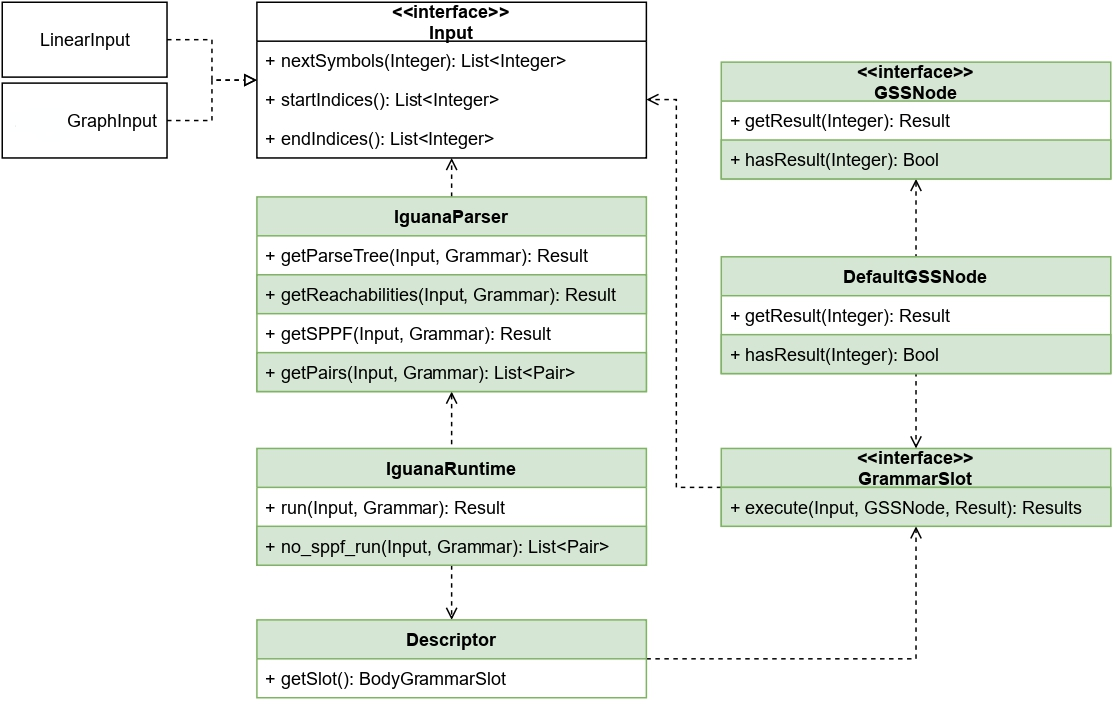
\includegraphics[width=0.95\textwidth]{figures/sppf_arch.jpg}
    \caption{Architecture of the solution}
    \label{fig:solution_architecture}
\end{figure}

The main parts of the solution are presented in figure~\ref{fig:solution_architecture}. To handle the scenario when SPPF construction is omitted almost all architecture elements were changed. The green color in this diagram marks the classes and methods that have been changed at this stage of the work. \texttt{Iguana Runtime} takes an \texttt{Input} and a context-free \texttt{Grammar} to produce the \texttt{Result}. The  \texttt{Result} is a key entity which should or should not contain SPPF information. \texttt{Input} abstracts a data structure with the ability to get the next symbols for the given position. One example of \texttt{Input} is \texttt{Graph}, in which the position is a vertex, and the next symbols are the labels of its outgoing edges. There was provided to use different forms of graph representation. Communication with the database is done using the Neo4j Native Java API. The way to create a database was changed. Now an embedded database is used. It means that it runs inside of the application and it is not used as an external service as it was earlier. Worth noting, the architecture is extensible, and one can provide their own implementation of \texttt{Graph} to enable context-free path querying for a new graph storage.
This section demonstrates the practical results of the proposed approach application. We introduce an easy-to-use implementation, specify some experimental details and describe currently available models. We compare our results with several popular tools and show the competitive power of our models.

\subsection{Tool}
The proposed approach was implemented as a Python console tool Genegram. Code, installation instructions, and documentation are available by link \linebreak \url{https://github.com/JetBrains-Research/Genegram}. This tool accepts a file with RNA sequences in fasta format and returns the connectivity tables (ct) for the corresponding secondary structures. We use an effective Python implementation of the parsing algorithm~\cite{Azimov:2018:CPQ:3210259.3210264} that shows high performance due to the GPGPU utilization and Keras~\cite{chollet2015keras} library with Tensorflow-GPU~\cite{tensorflow2015-whitepaper} framework for running the predictive model. Genegram tool allows to select different models and process sequences of lengths 1-200 containing only four canonical nucleotides.

\subsection{Setup}
The approach itself is quite flexible and Genegram tool provides a convenient environment for different experiments allowing to change both grammar and network. However, in the present work, we freeze grammar $G_0$ from figure~\ref{gram} and parallel ResNet architecture from figure~\ref{nn} with $k := 10$, $n := 4$. We consider only small RNAs (lengths from 1 to 200) due to the insufficient amount of longer sequences in biological databases and GPU storage limitations. Each sequence of $l$ nucleotides results in the image of size $l \times l$, therefore, images are grouped into batches by image size and cyclically duplicated until all batches have the same length. We use two data augmentation techniques on the training dataset: firstly, we mirror each image along the main diagonal (so that mirrored image represents the same sequence turned backwards), and secondly, we copy both regular and mirrored images twice. On this data, we run 10-fold cross-validation in order to choose the best train and validation split for each model.

The quality of the results is estimated by classical machine learning metrics calculated on the pixel-by-pixel difference between predicted and reference images. Further, we consider $TP$ (true positives, i.e. true white pixels), $FP$ (false positives, i.e. false white pixels), and $FN$ (false negatives, i.e. false black pixels) as numbers of right and wrong decisions among all contacts and calculate three following metrics for each image of some dataset. 

\begin{itemize} 
    \item $Precision = \displaystyle \frac{TP}{TP + FP}$ (proportion of correct contacts among all detected).
    \item $Recall = \displaystyle \frac{TP}{TP + FN}$ (proportion of detected contacts among all expected).
    \item $F1 = \displaystyle 2 * \frac{Precision * Recall}{Precision + Recall}$ (harmonic mean --- aggregation metrics).
\end{itemize}

The loss function is based on the idea of maximizing $F1$ score and that is to be achieved by minimizing the dataset mean $1 - F1$ through gradient descent. However, $F1$ is not differentiable as a function, so, we replace the sums of discrete integer values with a continuous sum of probabilities. Also, we charge our loss with two penalty coefficients responsible for huge dispersion between $Precision$ and $Recall$ for each image ($k1$) and the whole dataset ($k2$). Figure~\ref{loss} demonstrates the Python code for the currently used  $F1\_loss$ function that accepts two arguments: predicted image $y\_p$ and true image $y\_t$.

\begin{figure}[h]
\centering
\begin{lstlisting}[language=Python]
from keras import backend as K

def f1_loss(y_t, y_p):
    #normalize pixels values to [0, 1]
    y_t, y_p = K.minimum(y_t / 255, 1), K.minimum(y_p / 255, 1)
    #calculate differentiable versions of tw, fw and fb
    tw = K.sum(K.cast(y_t * y_p, 'float32'), axis=[1, 2, 3])
    fw = K.sum(K.cast((1 - y_t) * y_p, 'float32'), axis=[1, 2, 3])
    fb = K.sum(K.cast(y_t * (1 - y_p), 'float32'), axis=[1, 2, 3])
    #calculate precision and recall secure from zero division error
    prec = tw / (tw + fw + K.epsilon())
    rec = tw / (tw + fb + K.epsilon())
    #penalties for huge difference between precision and recall 
    #calculated for each image and whole dataset respectively
    k1 = 1 -  K.abs(prec- rec)
    k2 = 1 -  K.abs(K.mean(prec) - K.mean(rec))
    #calculate upgraded f1 score and return its mean value
    f1 = k1 * k2 * 2 * prec * rec / (prec + rec + K.epsilon()) 
    return 1 - K.mean(f1)
\end{lstlisting}
\caption{$F1\_loss$ function}
\label{loss}
\end{figure} 

For hyperparameters, we use Dropout after each residual unit to deal with overfitting, L2-regularization that also prevents overfitting and allows to search for complex data patterns, and Adagrad optimizer that automatically sets the learning rate and is known to be a powerful solution for sparse data processing.

For a comparative analysis of the results we selected six tools based on various concepts and algorithms. All of them demonstrate adequate speed and high accuracy, can handle pseudoknots and are easy to launch and use.

\begin{itemize}
    \item SPOT-RNA~\cite{singh2019rna} --- deep neural networks + transfer learning.
    \item Ipknot~\cite{sato2011ipknot} --- MEA + integer programming.
    \item Knotty~\cite{jabbari2018knotty} --- MFE + sparse dynamic programming.
    \item RNAstructure~\cite{bellaousov2013rnastructure} --- MFE + dynamic programming. 
    \item PknotsRG~\cite{reeder2007pknotsrg} --- MFE + Turner energy rules.
    \item HotKnots~\cite{ren2005hotknots} --- MFE + heuristic algorithm.
\end{itemize}

\subsection{Models}
In these conditions, we trained three identical networks on three different datasets and compared them with each other and with other tools by several criteria. All three models are available to use in the Genegram tool and the default model here is Genegram-main. Let us describe the specifics of each dataset, present the results of the best 10-fold cross-validation splits, and draw some conclusions.

\subsubsection{Genegram-main}
The first model was trained on data obtained from RNA STRAND database~\cite{andronescu2008rna} that is quite popular in different RNA analysis research due to its quality and usability. This database is an assembly of carefully curated and validated RNA sequences with secondary structures collected from different sources, and it contains only trustful structures obtained by reliable methods (laboratory or comparative). This database is supposed to provide the most representative sample of RNA secondary structures along with a guaranteed high quality of data which makes Genegram-main model trained on RNA STRAND the most general one for now, therefore, we set it as a default choice for our tool.

We selected 1091 sequences with lengths up to 200 and removed samples with gaps or inaccuracies in primary and secondary structures. The distribution of sequences lengths in the prepared dataset is demonstrated in figure~\ref{main_distr}. Neural network output images are grayscale and may contain multiple contacts, therefore, we applied binarization by threshold 0.6 with multiplets removal as postprocessing for this model and calculated the following metrics afterwards. Figure~\ref{main_f1} shows the estimation of Genegram-main and other six tools on validation set of size 109 by metrics $F1$. The shape of colored plots shows the density of $F1$ values, the red line represents its median result and the blue line corresponds to the mean one. It can be seen that Genegram-main has median $F1$ equal to 81 (as well as Knotty which is the second result after SPOT-RNA), and mean $F1$ equal to 70 that significantly exceeds the results of all competing tools except SPOT-RNA. The estimation on the same set by mean $Precision$ and $Recall$ metrics is presented in figure~\ref{main_pr}. Note that the binarization threshold allows us to slightly manipulate the balance between these two metrics and we choose it so that $F1$ mean value is the highest, even though it leads to a small excess of $Precision$ over $Recall$.

\begin{figure}[h]
\centering
    \subfloat[$F1$ distribution, mean, \\ and median on valid set]
        {\label{main_f1}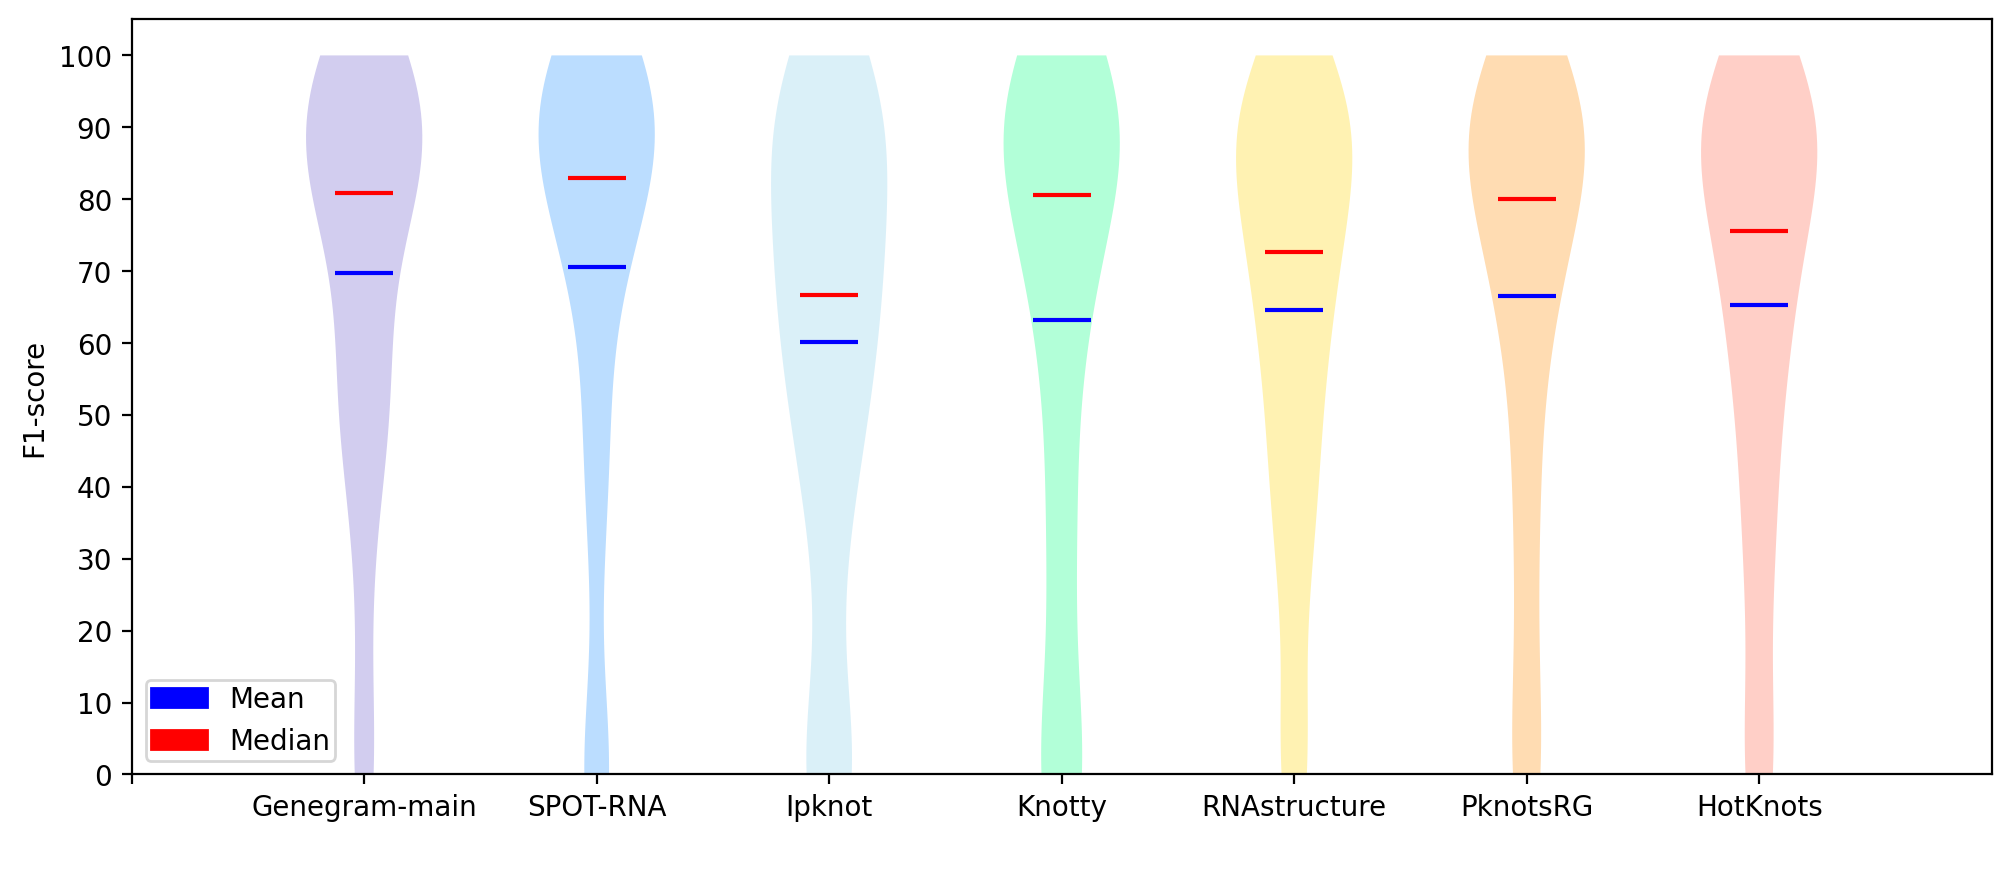
\includegraphics[width=.69\linewidth]{pics/plot_main_f1.png}}\hfill
    \subfloat[$Precision$ and $Recall$ mean on valid set]
        {\label{main_pr}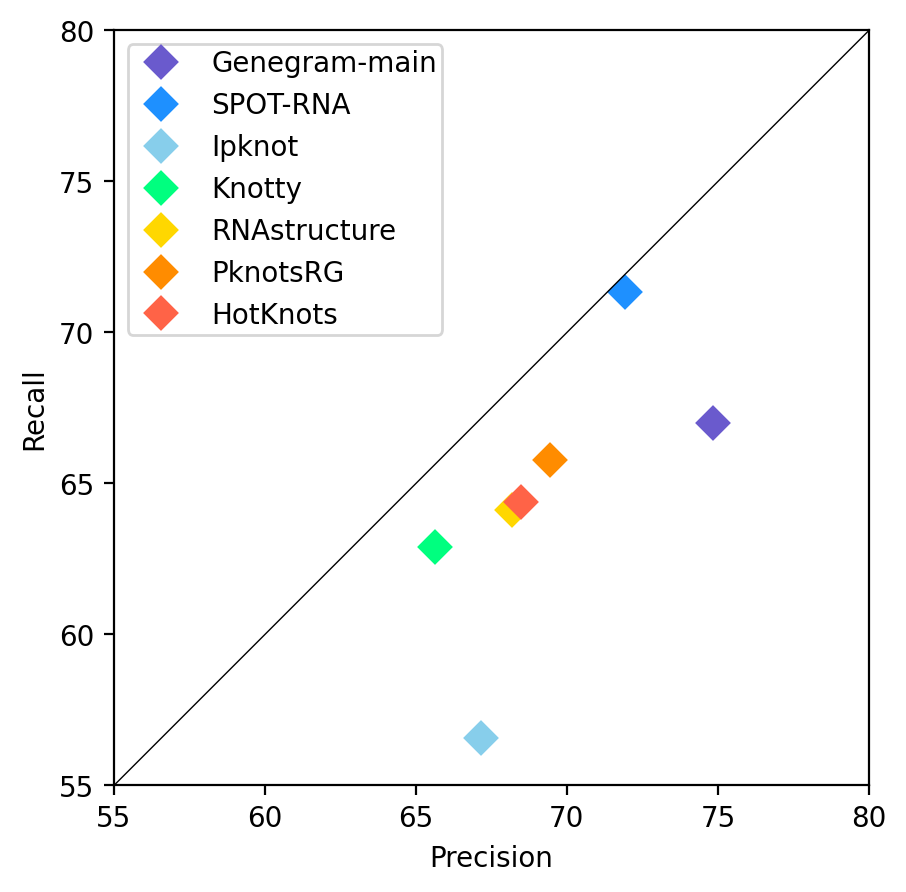
\includegraphics[width=.31\linewidth]{pics/plot_main_pr.png}}\par 
    \subfloat[Sequences lengths distribution on total set]
        {\label{main_distr}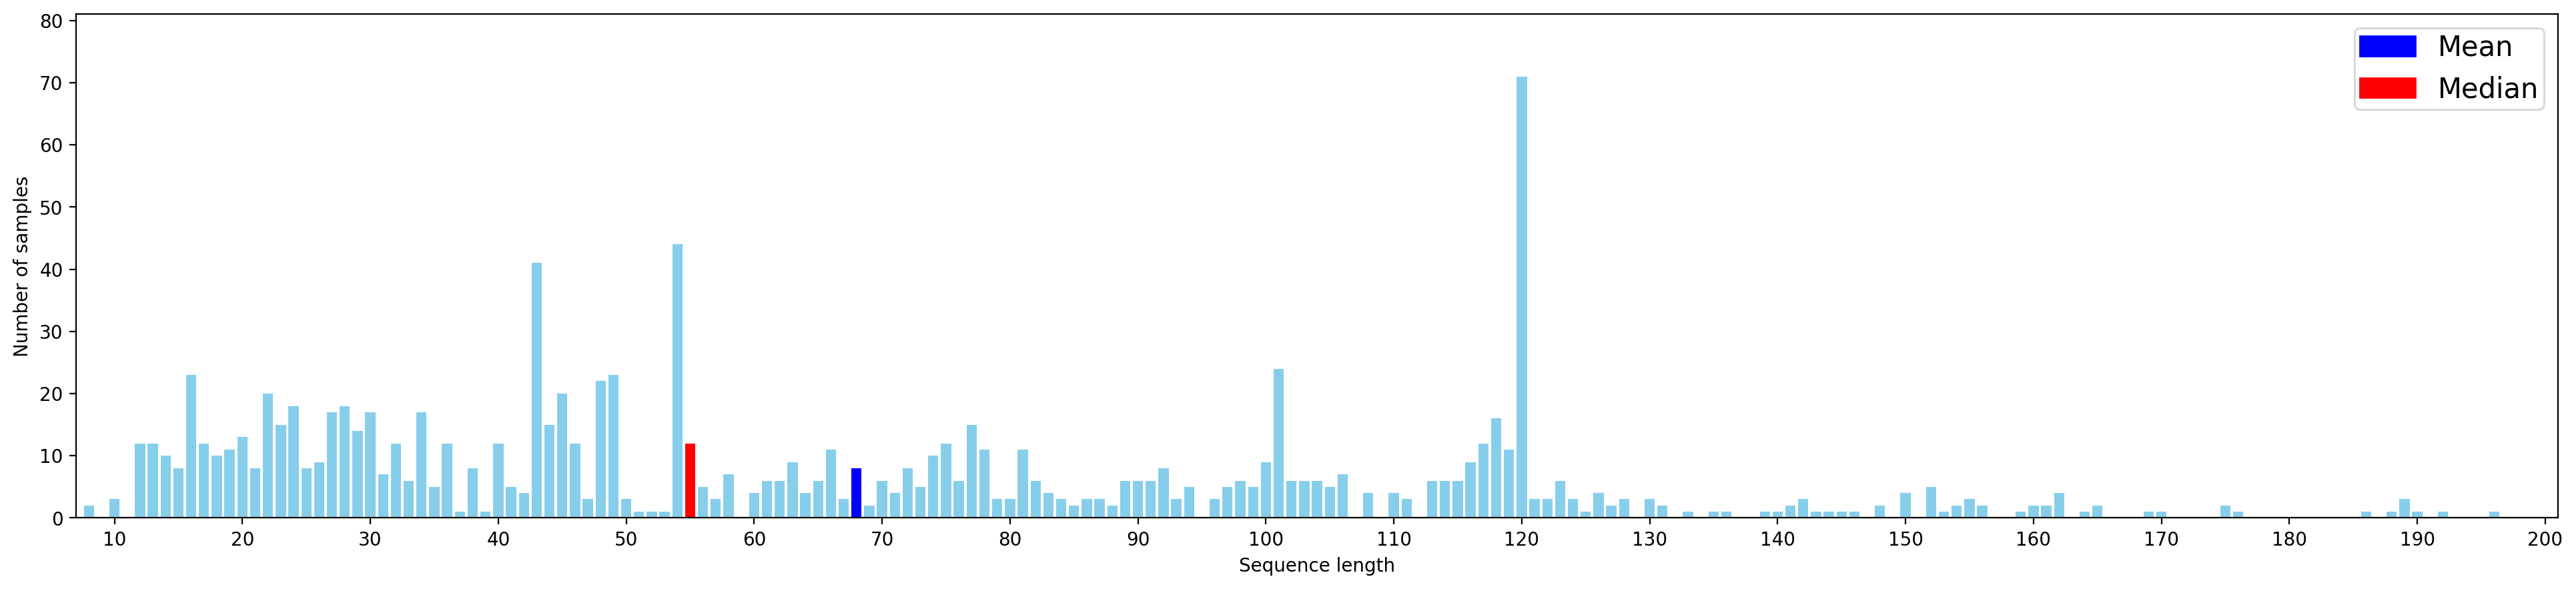
\includegraphics[width=\linewidth]{pics/plot_main_distr.png}}
\caption{Analysis of Genegram-main model compared with other tools }
\label{plots_main}
\end{figure}

All models were also estimated by several more specific functional criteria, such as pseudoknots prediction accuracy and sensitivity to different types of base pairs, so, table~\ref{table_main} demonstrates the results of these experiments. Considered validation set contained 11 pseudoknots and we calculated the number of correctly predicted contacts for each pseudoknot in each model output. The second column of table~\ref{table_main} shows the number of perfectly detected pseudoknots and the third column --- the number of ones that had up to 25\% extra or missing contacts. Clearly, pseudoknotted structures prediction is a non-trivial task for almost all models including Genegram-main. The other three columns of table~\ref{table_main} demonstrate how these tools handle different types of base pairs. Watson-Crick pairs are the most common and stable ones and it can be seen that all models have high enough canonical pairs prediction accuracy. Besides, it is known that wobble base pairs also have a biological role and regularly appear in real-world data, especially GU pair that has stability close to the Watson-Crick bonds. Our model slightly loses to other tools in GU pairs prediction, however, the great advantage of our approach is that it does not limit any types of pairs to be presented in neural network output (as well as SPOT-RNA that also uses neural networks), so, Genegram-main and SPOT-RNA are able to handle seven more wobble base pairs (AA, AC, AG, CC, CU, GG, UU), unlike other considered tools.

\begin{table}[h!]
\centering
\caption{Genegram-main and other models quality criteria measured on valid set}
\ra{1.4}
\begin{tabular}{@{}lccccccc@{}}\toprule
& \multicolumn{2}{c}{Pseudoknots} & \phantom{abc}& \multicolumn{3}{c}{Base pairs} \\
& No errors & 25\% errors  && Watson-Crick & GU & Others \\ \cmidrule{2-3} \cmidrule{5-7} 
Genegram-main  & 0 & 3 && 1067 & 68 & 53 \\
SPOT-RNA & 1 & 4 && 1190 & 134 & 39 \\
Ipknot & 0 & 1 && 939 & 92 & 0 \\
Knotty &1 & 3 && 1093 & 126 & 0 \\
RNAstructure & 1 & 1 && 1113 & 119 & 0 \\
PknotsRG & 1 & 5 && 1157 & 123 & 0 \\
HotKnots & 1 & 2 && 1113 & 112 & 0 \\
\bottomrule
Expected & 11 & 11 && 1650 & 185 & 135 \\
\bottomrule
\end{tabular}
\label{table_main}
\end{table}

\subsubsection{Genegram-pks}
Although the main model shows high results in general, it has poor pseudoknots prediction accuracy because RNA STRAND database contains only 86 sequences with pseudoknots and the neural network has not enough data to learn them, moreover, the amount of pseudoknots in the considered validation set is not enough to draw any conclusions. To improve this, we extended the previous dataset with sequences from Pseudobase~\cite{van2000pseudobase} database that is known to be a carefully built collection of pseudoknotted structures. Even though this database mostly contains not the whole sequences but only fragments with pseudoknots, we believe that the presence of such data in the training set may allow us to reach higher results in pseudoknots prediction.

We selected 1447 sequences having lengths up to 200 with no gaps or inaccuracies in primary and secondary structures and applied the same binarization by threshold 0.6 with multiplets removal as postprocessing. Note that both times we used 10-fold cross-validation on randomly shuffled data, so, Genegram-pks has separate from Genegram-main validation set, even though samples may intersect. Figure~\ref{pks_distr} shows the distribution of sequences lengths in total Genegram-pks dataset, figure~\ref{pks_f1} estimates all seven models on 145 validation sequences by $F1$ and figure~\ref{pks_pr} --- by $Precision$ and $Recall$ metrics. Genegram-pks is behind two tools by mean $F1$ value (70) and behind three tools by median (75) one, so, these results are quite competitive, however, Genegram-main was able to achieve the higher numbers.

\begin{figure}
\centering
    \subfloat[$F1$ distribution, mean, \\ and median on valid set]
        {\label{pks_f1}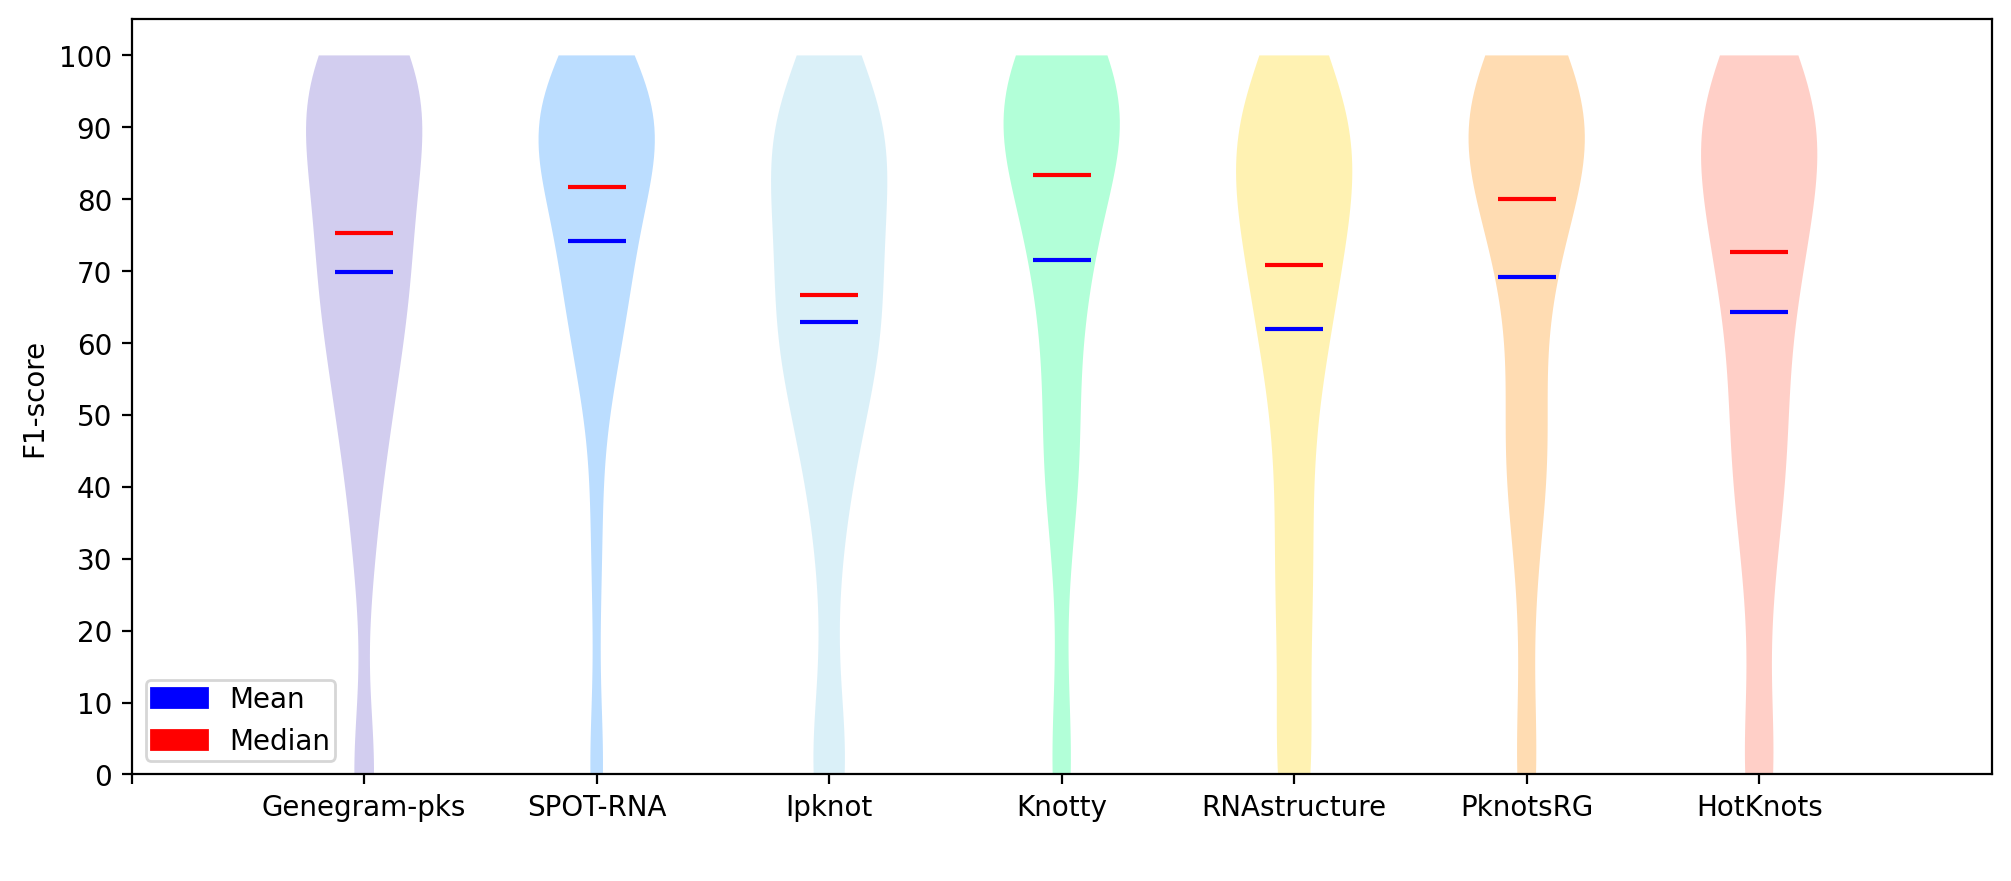
\includegraphics[width=.69\linewidth]{pics/plot_pks_f1.png}}\hfill
    \subfloat[$Precision$ and $Recall$ mean on valid set]
        {\label{pks_pr}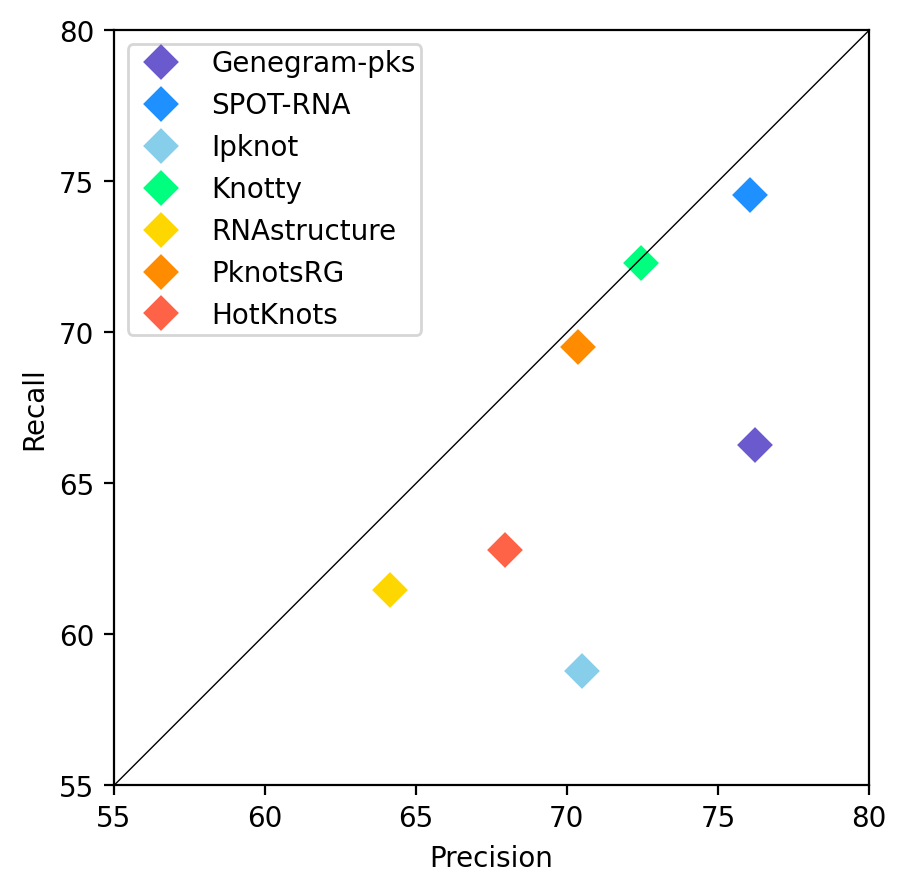
\includegraphics[width=.31\linewidth]{pics/plot_pks_pr.png}}\par 
    \subfloat[Sequences lengths distribution on total set]
        {\label{pks_distr}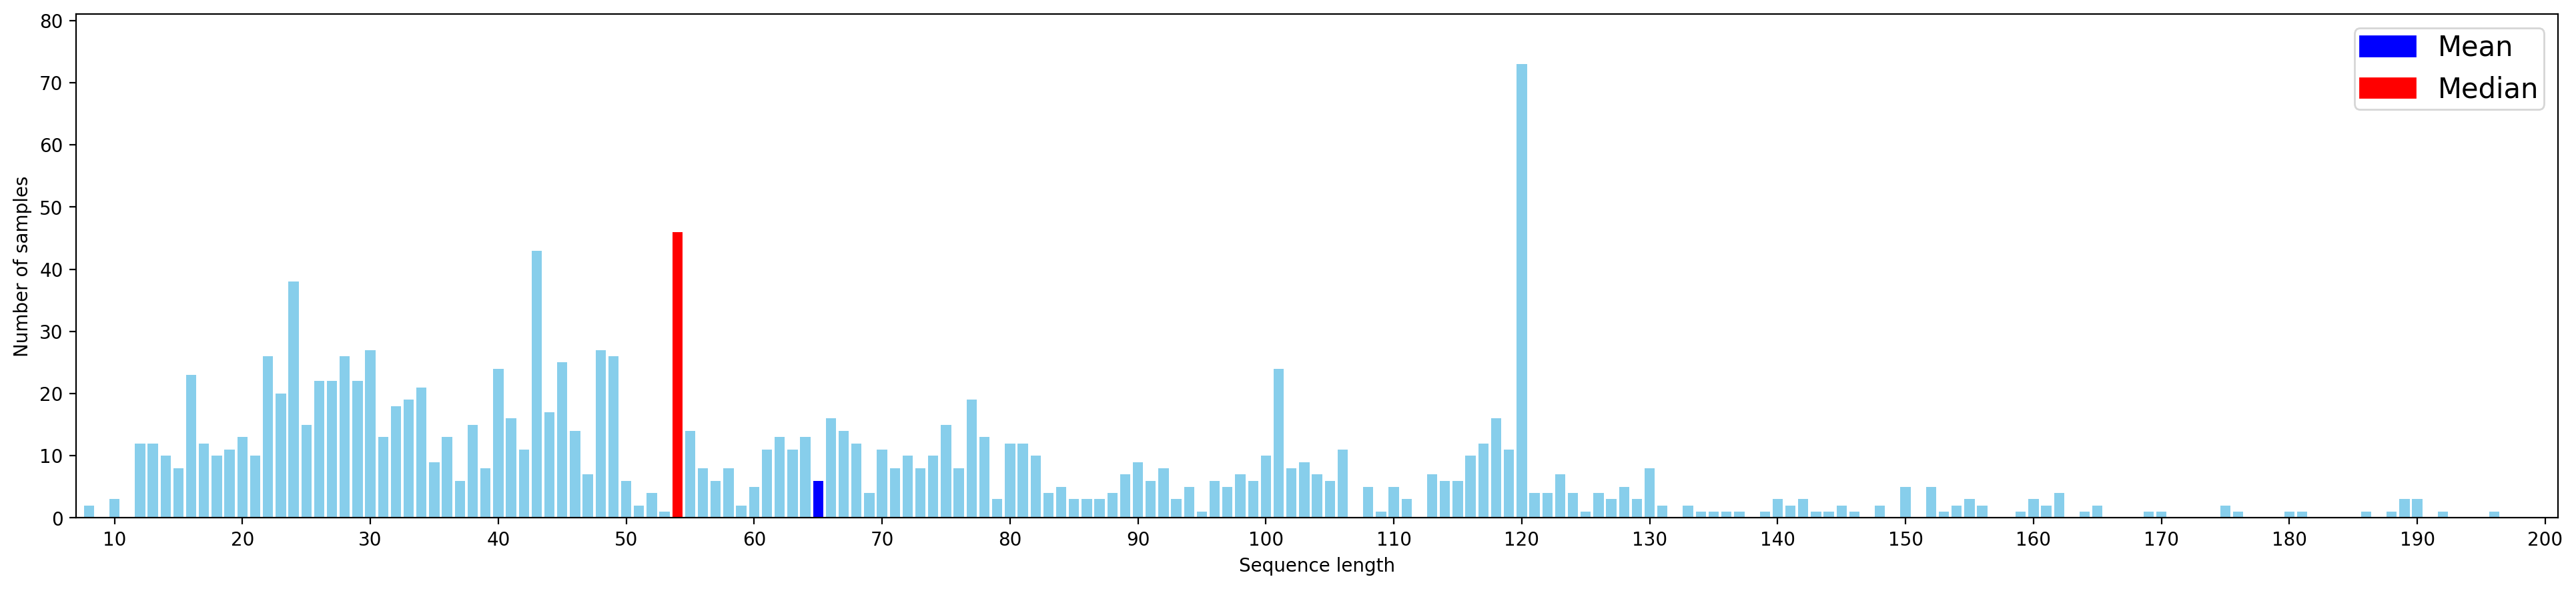
\includegraphics[width=\linewidth]{pics/plot_pks_distr.png}}
\caption{Analysis of Genegram-pks model compared with other tools }
\label{plots_pks}
\end{figure}

Similarly, we present the results of functional tests for this model and other tools in table~\ref{table_pks}. It can be seen that Watson-Crick pairs are predicted similarly to the main model, but wobble base pairs prediction accuracy decreased. However, the pseudoknotted structures processing was of particular interest in the context of Genegram-pks model and estimation by this criteria shows significant growth compared to the Genegram-main --- almost a quarter of all pseudoknots was detected perfectly, and about a half had small prediction errors. To sum up, this model generally losses to the main one, however, it shows very promising results in the aspect of pseudoknots detection being one of the best models for this problem.

\begin{table}
\centering
\caption{Genegram-pks and other models quality criteria measured on valid set}
\ra{1.4}
\begin{tabular}{@{}lccccccc@{}}\toprule
& \multicolumn{2}{c}{Pseudoknots} & \phantom{abc}& \multicolumn{3}{c}{Base pairs} \\
& No errors & 25\% errors  && Watson-Crick & GU & Others \\ \cmidrule{2-3} \cmidrule{5-7} 
Genegram-main  & 9 & 18 && 1628 & 61 & 47 \\
SPOT-RNA & 4 & 10 && 1893 & 173 & 71 \\
Ipknot & 2 & 5 && 1497 & 120 & 0 \\
Knotty & 11 & 20 && 1833 & 156 & 0 \\
RNAstructure & 3 & 7 && 1550 & 140 & 0 \\
PknotsRG & 11 & 20 && 1742 & 150 & 0 \\
HotKnots & 6 & 6 && 1621 & 143 & 0 \\
\bottomrule
Expected & 43 & 43 && 2407 & 258 & 156 \\
\bottomrule
\end{tabular}
\label{table_pks}
\end{table}

\subsubsection{Genegram-mps}
Another object that our approach allows to consider without any explicit definition is a multiplet that appears when base pair starts to form bonds with other bases or base pairs producing various topologies~\cite{bhattacharya2019going}. Multiplets are known to be functionally important, although, they are classified as tertiary structure features, so, secondary structure prediction tools are not usually able to handle them. In our terminology, multiplet would result in a reference image containing a set of white pixels where every two pixels have one equal coordinate, which makes multiplets processing possible in the terms of the considered approach.

For this experiment, we used data from PDB database~\cite{berman2000protein} that includes extracted from natural material RNA molecules with the corresponding crystallography results providing detailed structural information about secondary and tertiary interactions. This data tends to contain a lot of variability and complicated patterns, therefore, it creates more research possibilities but also makes it harder to learn. So, Genegram-mps is a network that was trained on data from the PDB database and for now, it is an experimental model that has possibilities in predicting more features, especially, multiplets. We selected 712 sequences with lengths up to 200 and kept samples with interactions with other molecules and up to 20\% unmodeled residues due to the insufficient amount of perfectly clean samples in this database. We used RNAView software~\cite{yang2003tools} to generate base pairs list from RNA crystallography files and extended $F1\_loss$ function with a penalty coefficient that considers the percentage of correctly predicted multiplets contacts in all images. Also, we applied a smaller binarization threshold of 0.45 for this model. Figure~\ref{mps_distr} demonstrates the distribution of sequences lengths in the whole dataset, figure~\ref{mps_f1} estimates all models on 71 validation sequences by $F1$ metrics and figure~\ref{mps_pr} --- by $Precision$ and $Recall$ metrics. Genegram-mps has a slightly lower $F1$ value than other tools, however, it shows the highest $Recall$ due to the fact that it is the only model that can predict multiplets. 

\begin{figure}
\centering
    \subfloat[$F1$ distribution, mean, \\ and median on valid set]
        {\label{mps_f1}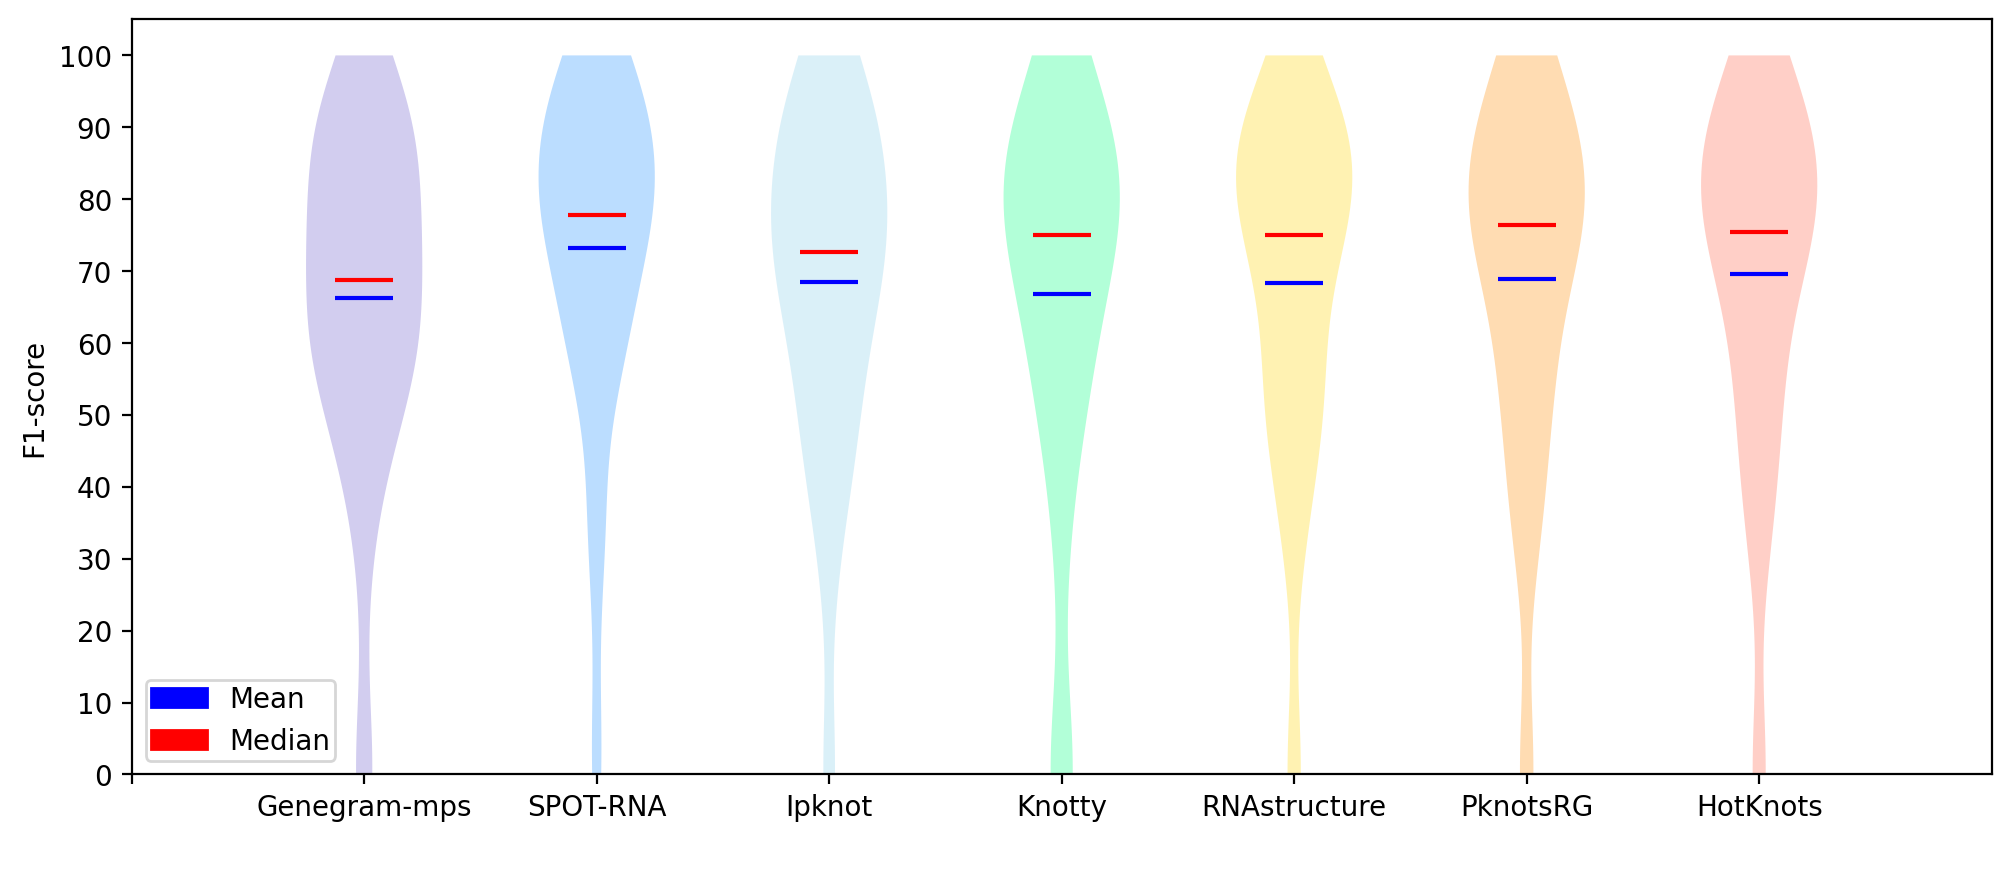
\includegraphics[width=.69\linewidth]{pics/plot_mps_f1.png}}\hfill
    \subfloat[$Precision$ and $Recall$ mean on valid set]
        {\label{mps_pr}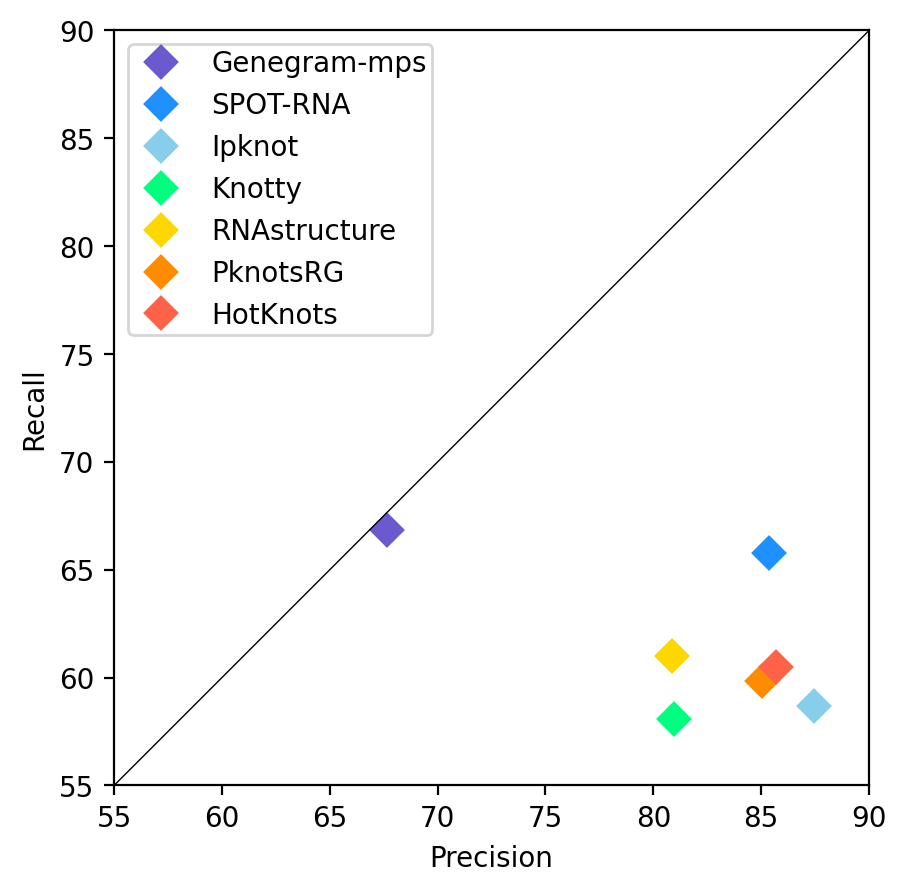
\includegraphics[width=.31\linewidth]{pics/plot_mps_pr.png}}\par 
    \subfloat[Sequences lengths distribution on total set]
        {\label{mps_distr}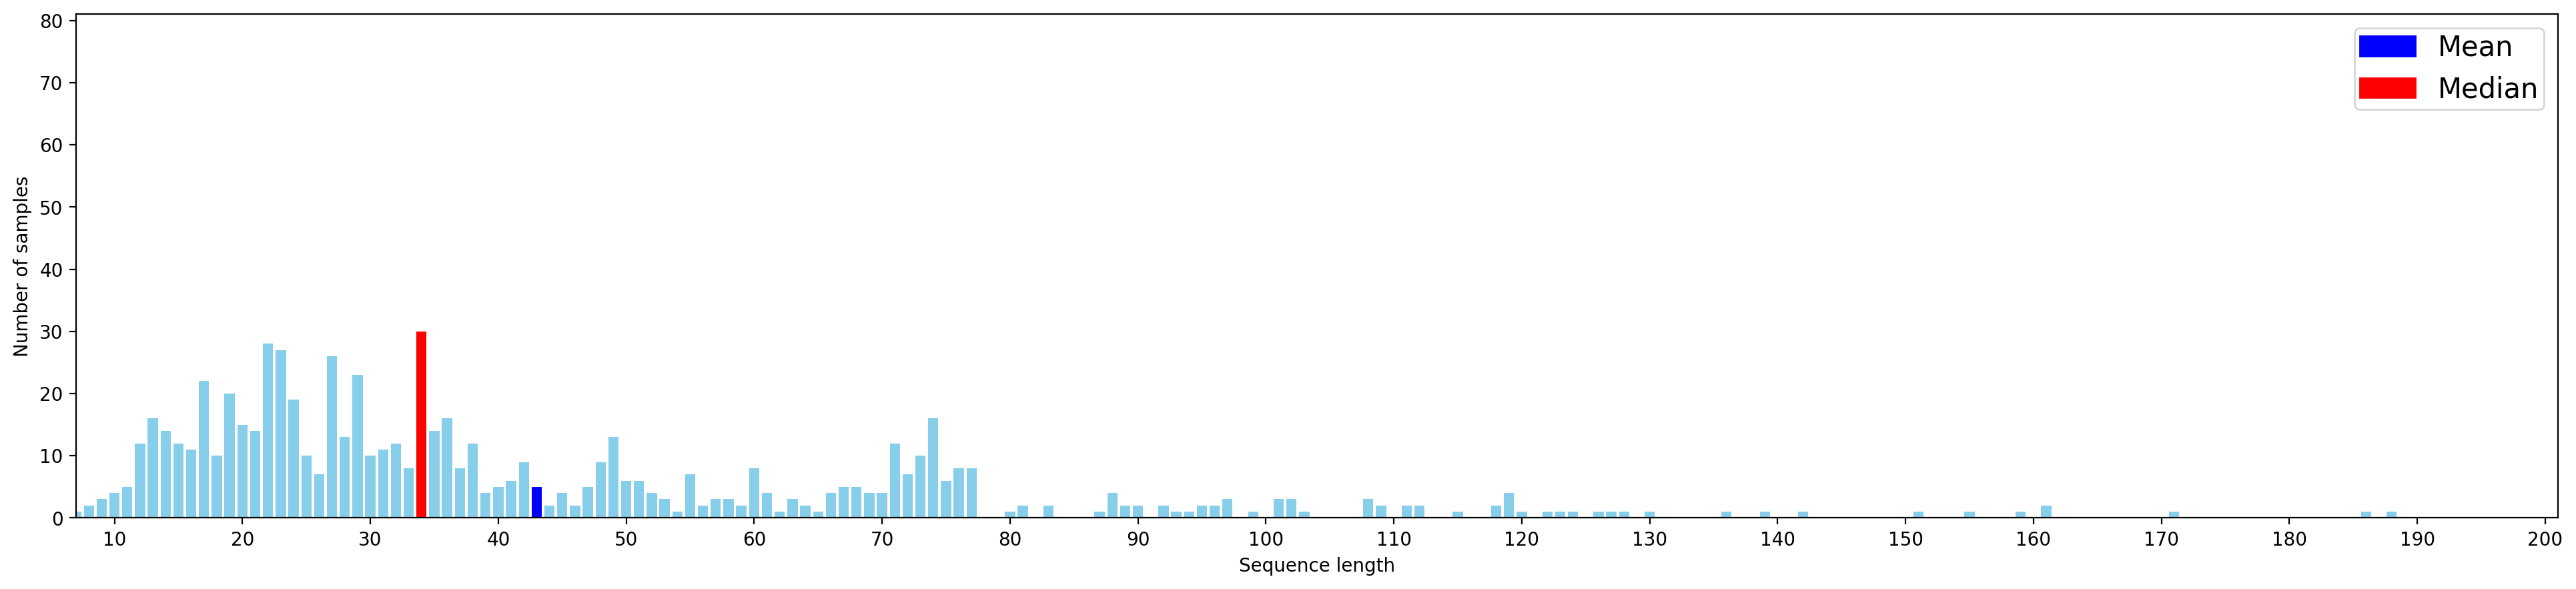
\includegraphics[width=\linewidth]{pics/plot_mps_distr.png}}
\caption{Analysis of Genegram-mps model compared with other tools }
\label{plots_pks}
\end{figure} 

As for functional tests, we similarly measured the prediction quality for three types of base pairs (table~\ref{table_mps}). Contacts belonging to multiplets are usually unstable, therefore, the ability of Genegram-mps model to predict multiplets resulted in high prediction accuracy for uncanonical base pairs. The definition of pseudoknot in the context of the multipletted structures is quite confusing, so, the estimation of pseudoknots was not run in this case. Instead of this, we provide the results of multiplets prediction. Note that there can be different ways of multiplets estimation and we choose two options for analysis: multiplets contacts (the amount of correct predictions among all contacts belonging to all multiplets in dataset) and multiplets pairs (the amount of correctly detected pairs $(i_1, j_1)$, $(i_2, j_2)$, where $i_1 = i_2$ or $i_1 = j_2$ or $j_1 = i_2$ or $j_1 = j_2$). The results of these tests are presented in the same table~\ref{table_mps}. It can be seen that all tools except Genegram are able to predict at most one contact of the multiplet pair and Genegram-mps model not only shows the highest contacts prediction score but also detects several paired interactions. However, the numbers are questionable so far, thus we introduce this model as a discussion about the possibilities of our approach rather than a final result.

\begin{table}[h!]
\centering
\caption{Genegram-mps and other models quality criteria measured on valid set}
\ra{1.4}
\begin{tabular}{@{}lccccccc@{}}\toprule
& \multicolumn{2}{c}{Multiplets} & \phantom{abc}& \multicolumn{3}{c}{Base pairs} \\
& Contacts & Pairs  && Watson-Crick & GU & Others \\ \cmidrule{2-3} \cmidrule{5-7} 
Genegram-mps  & 125 & 15 && 666 & 64 & 77 \\
SPOT-RNA & 101 & 0 && 680 & 64 & 44 \\
Ipknot & 67 & 0 && 630 & 56 & 0 \\
Knotty & 79 & 0 && 651 & 61 & 0 \\
RNAstructure & 73 & 0 && 643 & 62 & 0 \\
PknotsRG & 70 & 0 && 653 & 55 & 0 \\
HotKnots & 75 & 0 && 656 & 58 & 0 \\
\bottomrule
Expected & 448 & 395 && 863 & 132 & 316 \\
\bottomrule
\end{tabular}
\label{table_mps}
\end{table}

\subsubsection{Global tests}
In the previous sections we estimated three Genegram models separately on their validation sets and in this section, we provide some global tests for all the tools.

Due to the similar composition of training and validation sets for each model, the high results on validation make no reference to the general model quality, therefore, we downloaded several comparative and laboratory RNA secondary structure databases and evaluated Genegram models along with other tools on such data. These databases do not contain only purely selected structures, moreover, huge comparative databases usually aggregate a lot of homologous sequences with repetitive structural patterns, however, this experiment should check all models behavior on row data from various sources as opposed to the careful estimation on clean structures presented in the previous sections. We selected the following databases: CRW~\cite{cannone2002comparative}, Sprinzl~\cite{sprinzl1998compilation}, SRP~\cite{zwieb1992signal}, Rfam~\cite{griffiths2003rfam}, PDB~\cite{berman2000protein} (only single-chain samples without unmodelled bases) and Pseudobase~\cite{van2000pseudobase}. Note that most of these samples are completely new, however, some sequences or even databases could be previously used for some models training (e.g. Pseudobase was included in Genegram-pks training set). Table~\ref{table_all} represents the estimation of three Genegram models along with other tools by mean $F1$ score on all databases and the last column shows the mean $F1$ value among total samples. It can be seen that in most cases our models show adequate numbers regarding other tools, so, we can state that all neural networks generalize well on new datasets.

\begin{table}
\centering
\caption{All models estimation by $F1$ metrics on different databases}
\ra{1.4}
\begin{tabular}{@{}lcccccccc@{}}\toprule
& CRW & Sprinzl & SRP & Rfam & PDB & Pseudobase  & All data \\ \cmidrule{2-8} 
Genegram-main  & 69 & 73 & 59 & 43 & 74 & 42 & 69 \\
Genegram-pks  & 66 & 72 & 56 & 48 & 74 & 81 & 68 \\
Genegram-mps  &  &  &  &  &  &  &  \\
SPOT-RNA & 89 & 88 & 65 & 72 & 81 & 70 & 87 \\
Ipknot & 74 & 79 & 49 & 64 & 76 & 59 & 75 \\
Knotty & 74 & 75 & 63 & 63 & 79 & 76 & 74 \\
RNAstructure & 66 & 69 & 56 & 64 & 77 & 62 & 67 \\
PknotsRG & 62 & 61 & 65 & 66 & 79 & 77 & 62 \\
HotKnots & 61 & 60 & 66 & 66 & 78 & 61 & 61 \\
\bottomrule
Total samples & 11606 & 8777 & 360 & 1043 & 290 & 357 & 22433 \\
\bottomrule
\end{tabular}
\label{table_all}
\end{table}

Finally, we measured the time required for each tool to process fasta file with 100 RNA sequences and return secondary structure prediction for each sequence in its default output format. These tests were carried out on the workstation with the following characteristics: Ubuntu 20.04.2 LTS, Intel Core i5-10210U CPU 1.60GHz, NVIDIA GeForce MX250 GPU, and 7.5 GB RAM. We prepared two datasets by randomly selecting sequences from RNA STRAND database: the first set contained 100 sequences having lengths up to 100 and the second one --- 100 sequences with lengths up to 200. Table~\ref{table_time} shows the results of a performance experiment for such two fasta files. Genegram and SPOT-RNA were launched on GPU and the other tools have only CPU versions. It can be seen that the elapsed time spread among tools is quite big, moreover, several tools significantly lose in performance while processing longer sequences since various secondary structure prediction techniques may have completely different algorithmic complexity. However, Genegram shows an adequate performance due to the effective use of GPGPU in the parsing algorithm as well as in the neural network.

\begin{table}
\centering
\caption{Tools time performance on 100 sequences}
\ra{1.4}
\begin{tabular}{@{}lccc@{}}\toprule
& \multicolumn{2}{c}{\phantom{abc}  \phantom{abc}  \phantom{abc} Elapsed time, seconds}  \\
& Lengths 1-100 && Lengths 1-200  \\ \cmidrule{2-2} \cmidrule{4-4} 
Genegram & 28 && 39 \\
SPOT-RNA & 68 && 235 \\
Ipknot & 1 && 1 \\
Knotty & 283 && 3050 \\
RNAstructure & 10 && 15 \\
PknotsRG & 15 && 95 \\
HotKnots & 37 && 366 \\
\bottomrule
\end{tabular}
\label{table_time}
\end{table}
\section{Модернизация набора данных \textsc{CFPQ\_Data}}

В результате обзора предметной области в проект \textsc{CFPQ\_Data} были внесены следующие изменения.
\begin{itemize}
    \item Было изменено стандартное представление графов и грамматик.
    \item Обновлено и расширено множество функций, предоставляемых проектом.
    \item Доступ к набору данных изменен с интерфейса командной строки на Python пакет, опубликованный в PYPI\footnote{Python пакет <<\textsc{CFPQ\_Data}>>: \url{https://pypi.org/project/cfpq-data/}, дата последнего доступа --- 04.06.2021}.
    \item Добавлено и автоматизировано интеграционное тестирование.
    \item Обновлен веб-сайт и автоматизирована его публикация.
\end{itemize}

\subsection{Представление данных}

Представление графа в виде множества записей вида <<объект, предикат, субъект>> хотя и идеально соответствует структуре помеченного графа и позволяет компактным образом хранить граф, но не подходит для исследования и манипулирования графами.
Именно поэтому в качестве стандартного представления помеченного графа выбран класс <<MultiDiGraph>> из проекта <<networkx>>\footnote{GitHub репозиторий <<networkx>>: \url{https://github.com/networkx/networkx}, дата последнего доступа --- 04.06.2021}, который является одним из наиболее известных проектов для работы с графами, хорошо задокументирован и имеет внушительное сообщество.
Такое архитектурное решение позволяет применять к графам, имеющимся в \textsc{CFPQ\_Data}, весь богатый арсенал функций из проекта <<networkx>>, что несомненно упрощает их исследование и манипулирование ими.

По тем же причинам, в качестве стандартного представления кон\-текстно-свобод\-ной грамматики выбран класс <<CFG>> из проекта <<py\-form\-lang>>\footnote{GitHub репозиторий <<py\-form\-lang>>: \url{https://github.com/Aunsiels/pyformlang}, дата последнего доступа --- 04.06.2021}, который является одним из наиболее известных проектов для работы с формальными языками и, в том числе, с контекстно-свободными грамматиками.
Кроме того, было реализовано представление контекстно-свободной грамматики с помощью рекурсивного автомата~\cite{RSM}.

\subsection{Архитектура}

Все предоставляемые для работы с графами и грамматиками функции выделены в один пакет <<\textsc{CFPQ\_Data}>>.

\begin{figure}[h]
    \centering
    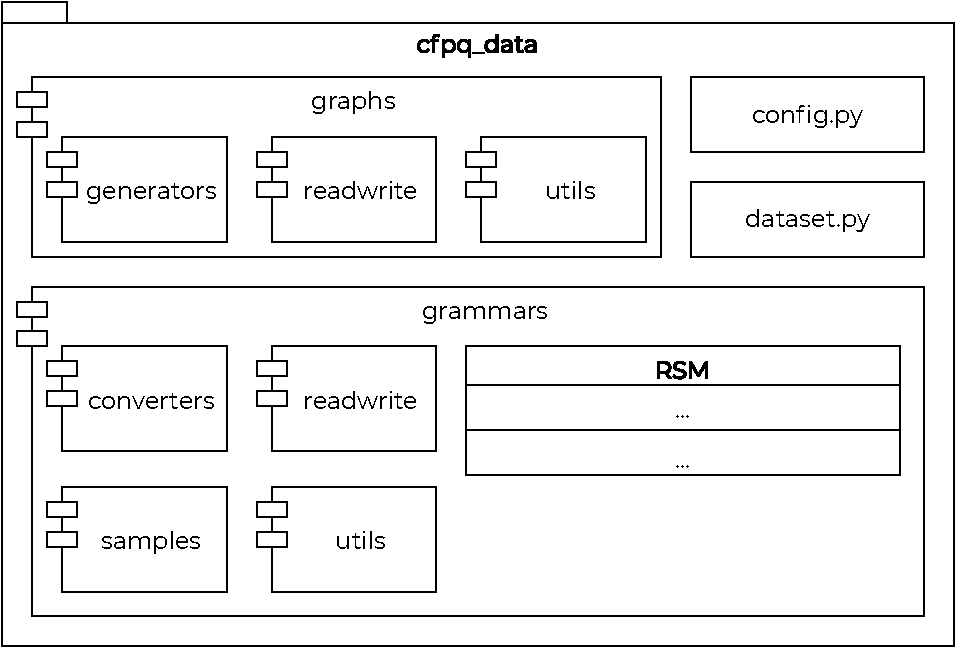
\includegraphics[width=\textwidth]{img/architecture_new.pdf}
    \caption{Новая архитектура \textsc{CFPQ\_Data}}
\end{figure}

Функции для манипулирования графами собраны в модуле <<graphs>>, который состоит из трех подмодулей.
\begin{itemize}
    \item В подмодуле <<generators>> реализованы функции генерации синтетических графов.
    \item В подмодуле <<readwrite>> реализованы функции чтения и записи графов, представленных в формате RDF и в формате троек <<вершина, метка ребра, вершина>>.
    \item В подмодуле <<utils>> реализованы функции для трансформации графов.
\end{itemize}

Функции для манипулирования грамматиками собраны в модуле <<grammars>>, который состоит из четырех подмодулей.
\begin{itemize}
    \item В подмодуле <<converters>> реализованы функции конвертации кон\-текстно-свобод\-ной грамматики между различными представлениями.
    \item В подмодуле <<readwrite>> реализованы функции чтения и записи кон\-текстно-свобод\-ной грамматики, представленной в различных форматах.
    \item В подмодуле <<samples>> реализованы примеры кон\-текстно-свобод\-ных запросов для соответствующих помеченных графов из <<graphs>>.
    \item В подмодуле <<utils>> реализованы функции для трансформации грамматик.
\end{itemize}

В файле <<dataset.py>> фиксируется информация о графах, сохраненных в \textsc{CFPQ\_Data}, соответствующая версии пакета, а в файле <<config.py>> фиксируется конфигурация доступа пакета к набору данных.

Также, с помощью GitHub Actions\footnote{GitHub Action интеграционного тестирования: \url{https://github.com/JetBrains-Research/CFPQ_Data/actions/workflows/tests.yml}, дата последнего доступа --- 04.06.2021} было реализовано интеграционное тестирование полученного пакета на юнит-тестах на различных операционных системах, с последующим сбором информации о покрытии кода.

\subsection{Документация}
Все предоставляемые пользователю функции были снабжены документацией, публикация которой добавлена в новой версии веб-сайта проекта.
Также на веб-сайт были добавлены следующие страницы.
\begin{itemize}
    \item Страница\footnote{<<Dataset>>: \url{https://jetbrains-research.github.io/CFPQ_Data/dataset/index.html}, дата последнего доступа --- 04.06.2021} с описанием графов из набора данных \textsc{CFPQ\_Data}.
    \item Страница\footnote{<<Install>>: \url{https://jetbrains-research.github.io/CFPQ_Data/install.html}, дата последнего доступа --- 04.06.2021} с руководством по установке пакета.
    \item Страница\footnote{<<Tutorial>>: \url{https://jetbrains-research.github.io/CFPQ_Data/tutorial.html}, дата последнего доступа --- 04.06.2021} с руководством помогающим начать пользоваться пакетом.
    \item Страница\footnote{<<Reference>>: \url{https://jetbrains-research.github.io/CFPQ_Data/reference/index.html}, дата последнего доступа --- 04.06.2021} с документацией всех функций, имеющихся в пакете.
    \item Страница\footnote{<<About>>: \url{https://jetbrains-research.github.io/CFPQ_Data/about.html}, дата последнего доступа --- 04.06.2021} с информацией о группе разработчиков проекта.
    \item Страница\footnote{<<License>>: \url{https://jetbrains-research.github.io/CFPQ_Data/license.html}, дата последнего доступа --- 04.06.2021} с лицензией проекта.
\end{itemize}

Также было сохранено индексирование проекта в Google Dataset Search и автоматизирована публикация сайта на GitHub Pages с помощью GitHub Actions\footnote{GitHub Action публикации веб-сайта: \url{https://github.com/JetBrains-Research/CFPQ_Data/actions/workflows/deploy_docs.yml}, дата последнего доступа --- 04.06.2021}.

\setmonofont[Mapping=tex-text]{CMU Typewriter Text}
\bibliographystyle{ugost2008ls}
\bibliography{diploma.bib}
\end{document}
